% =====================================================================
% Actionable Futures -> ICLR 2027 submission skeleton
% Plan: PAPER_WRITING_PLAN_2026-08-12.md
% Build: latexmk -pdf main.tex   (or `make`)
% =====================================================================
\documentclass{article}
\usepackage{iclr2027_conference}
% \iclrfinalcopy   % uncomment for camera-ready (de-anonymize)

\usepackage[utf8]{inputenc}
\usepackage[T1]{fontenc}
\usepackage{hyperref}
\usepackage{url}
\usepackage{graphicx}
\usepackage{booktabs}
\usepackage{multirow}
\usepackage{float}
\usepackage{amsmath,amsfonts,amssymb}
\usepackage{xcolor}
\usepackage{subcaption}
\input{math_commands.tex}

% Experiment placeholders in the internal draft. Remove before submission.
\newcommand{\exptodo}[2]{\par\noindent\textcolor{red}{\textbf{[EXP-TODO #1]} #2}}
\newcommand{\exptodoid}[1]{\textcolor{red}{\textbf{TODO #1}}}

% ---------- centralized numbers: update ONLY numbers.tex after G1/G2 ----------
% =====================================================================
% CENTRALIZED NUMBERS — single source of truth for all quantitative claims.
% Update here after each gate; text/tables reference these macros.
% Claim discipline (roadmap 4.16): aggregate diffs < 1.5pt are NOT claimable;
% all main-table numbers must be multi-seed with std.
% =====================================================================

% ---------- LIBERO-10, LaWAM stack (multi-seed, same-protocol) ----------
\newcommand{\noWMtSix}{76.5}          % no-WM baseline t6 (24-route seed protocol)
\newcommand{\lmwmTSix}{85.0}          % dual2q / tsched t6 (std 1.7--2.4)
\newcommand{\tSixGain}{+8.5}          % p<0.001, t~6  — THE robust guidance gain
\newcommand{\aggTsched}{95.22}        % n=8, ±0.91
\newcommand{\aggTschedStd}{0.91}
\newcommand{\aggDualQ}{94.80}         % n=4, ±0.71
\newcommand{\aggDualQStd}{0.71}
\newcommand{\aggBaselineArmB}{94.20}  % ±0.97 n=4 (E2 2026-07-24). 旧单评 96.4=噪声上尾, 弃用
\newcommand{\armBtSix}{82.5}          % ±3.8 (E2) — t6 分解: no-WM 76.5 → LaWM 82.5 (+6.0) → LMWM 85.0 (+2.5)
\newcommand{\armBtEight}{89.5}        % ±12.4 (E2, seed1=68!) — 基线 t8 也高方差, "LMWM伤t8"在LaWAM侧不成立
\newcommand{\tSixGainWM}{+6.0}        % 任何未来条件化(LaWM t+7) vs no-WM
\newcommand{\tSixGainMS}{+2.5}        % milestone 特异边际 (LMWM vs LaWM), 弱显著待更多seed
\newcommand{\tEightDualQ}{94}         % 2Q restores t8 from 90 (E1 dual) — capacity effect
% ---------- residual V8 (G1 locked for LIBERO-10; full 4-suite is diagnostic) ----------
\newcommand{\aggResid}{95.75}   % ±0.76 n=8 定稿 (6×NorthE-H20 + 2×gf0-A100, 同协议egl; seed{0,2,3,5,6,7,8,9})
\newcommand{\aggResidStd}{0.76}   % Δ+1.55 vs armB 94.20±0.97, Welch t≈2.80 → 过1.5声称线 ✅
\newcommand{\tSixResid}{87.5}    % ±3.8 n=8 — 指引 +5.0 vs armB 82.5; t9=90.8±2.7 (+4.8)
\newcommand{\tEightResid}{87.0}  % ±6.3 n=8 — 方差内 (armB 89.5±12.4); t7=100±0 满

% ---------- LIBERO full 4-suite honesty table (2026-07-28 status) ----------
\newcommand{\fourNowmAvg}{97.24}
\newcommand{\fourAbsAvg}{96.58}
\newcommand{\fourResidAvg}{96.90}
\newcommand{\fourShapeBAvg}{97.24}
\newcommand{\fourAbsDelta}{-0.62}
\newcommand{\fourResidDelta}{-0.30}
\newcommand{\fourShapeBDelta}{0.00}
\newcommand{\nowmLTen}{94.55}
\newcommand{\nowmLTenStd}{0.50}
\newcommand{\shapeBLTen}{95.30}
\newcommand{\shapeBLTenStd}{0.77}
\newcommand{\nowmGoal}{98.3}
\newcommand{\residGoal}{97.80}
\newcommand{\residGoalStd}{0.28}
\newcommand{\shapeBGoal}{98.00}
\newcommand{\shapeBGoalStd}{0.85}
\newcommand{\nowmObject}{99.8}
\newcommand{\residObject}{99.65}
\newcommand{\residObjectStd}{0.19}
\newcommand{\shapeBObject}{99.80}
\newcommand{\shapeBObjectStd}{0.23}
\newcommand{\nowmSpatial}{96.3}
\newcommand{\absSpatial}{93.3}
\newcommand{\residSpatial}{94.4}
\newcommand{\residSpatialStd}{0.84}
\newcommand{\shapeBSpatial}{95.85}
\newcommand{\shapeBSpatialStd}{1.18}

% ---------- pi05 stack (cross-architecture replication, 4 routes x 50) ----------
\newcommand{\piBase}{93.87}           % A0 baseline aggregate
\newcommand{\piExt}{93.07}            % A1 external DINOv3 hint
\newcommand{\piOwn}{93.70}            % A2 own-space So400m hint
\newcommand{\piOwnSuffix}{94.20}      % A2-suffix (only config above baseline)
\newcommand{\harmDifficultyCorrExt}{+0.66}   % ⚠DEMOTED(N5): CI跨0, 单离群t8驱动 — 正文不得作定律引用
\newcommand{\harmDifficultyCorrOwn}{+0.06}   % own-space: flat
\newcommand{\precDeltaExt}{-1.48}     % precision-task mean delta, external space
\newcommand{\precDeltaOwn}{-0.38}     % precision-task mean delta, own space
\newcommand{\tEightHarmExt}{-10.0}    % A1 on hardest precision task

% ---------- residual discriminability (mechanism) ----------
\newcommand{\residCV}{1.1}            % residual target trajectory CV
\newcommand{\absCV}{0.12}             % absolute target trajectory CV  (~10x)
\newcommand{\redundancyPct}{95\%}     % v3: FULL-CORPUS (1693ep, 4 suites, 100% episodes consistent); old per-ep estimate 86%
\newcommand{\residDiscrim}{15$\times$} % corpus-level residual-vs-absolute discriminability (per-ep examples ~10x)
\newcommand{\shapeBFrom}{93.2}        % spatial suite under absolute targets (shared-encoder gradients)
\newcommand{\shapeBTo}{95.9}          % spatial after WM-gradient detach (shapeB A/B); no-WM ref 96.5

% ---------- intrinsic recurrence signal ----------
\newcommand{\intrinsicGain}{2.1$\times$}  % r-ridge vs boundary forward gain

% ---------- RoboTwin all6 v2 (4 simulator seeds x 50 episodes/task) ----------
\newcommand{\rtNoWM}{91.1}
\newcommand{\rtLocal}{86.6}
\newcommand{\rtAbsolute}{89.2}
\newcommand{\rtResidual}{87.9}
\newcommand{\rtIsolation}{89.4}
\newcommand{\rtCombo}{89.2}
\newcommand{\rtLocalDelta}{-4.5}
\newcommand{\rtAbsoluteDelta}{-1.9}
\newcommand{\rtResidualDelta}{-3.2}
\newcommand{\rtIsolationDelta}{-1.7}
\newcommand{\rtComboDelta}{-1.9}
\newcommand{\rtStackThreeNoWM}{90.5}
\newcommand{\rtStackThreeAbsolute}{96.5}
\newcommand{\rtStackThreeResidual}{99.5}
\newcommand{\rtLocalSeedB}{86.75}
\newcommand{\rtComboSeedB}{88.92}

% ---------- pi0.5 RoboTwin internal matrix ----------
\newcommand{\piRTAZero}{35.50}
\newcommand{\piRTAOne}{41.17}
\newcommand{\piRTATwoAbs}{48.75}
\newcommand{\piRTATwoResid}{43.83}
\newcommand{\piRTAThree}{49.58}
\newcommand{\piRTAThreeVsZero}{+14.08}
\newcommand{\piRTAThreeVsResid}{+5.75}
\newcommand{\piRTAThreeVsAbs}{+0.83}
\newcommand{\piRTPublic}{78.42}

% ---------- pi0.5-preserving predictive adapter, seed-1000 screen ----------
\newcommand{\pOneAZero}{69.00}
\newcommand{\pOneNormal}{82.42}
\newcommand{\pOneZero}{78.50}
\newcommand{\pOneShuffled}{81.17}
\newcommand{\pOneMasked}{78.00}
\newcommand{\pOneVsAZero}{+13.42}
\newcommand{\pOneVsShuffled}{+1.25}
\newcommand{\rOneCrave}{68.67}
\newcommand{\rOneCombined}{62.92}
\newcommand{\rOneCombinedVsAZero}{-6.08}
\newcommand{\rOneCombinedVsCrave}{-5.75}

% ---------- outcome-calibrated demonstration weighting, seed-1000 screen ----------
\newcommand{\rFourOrdinary}{74.25}
\newcommand{\rFourCrave}{71.08}
\newcommand{\rFourTerminal}{77.58}
\newcommand{\rFourVsOrdinary}{+3.33}
\newcommand{\rFourVsCrave}{+6.50}
\newcommand{\rFourRepOrdinary}{72.14}
\newcommand{\rFourRepCrave}{71.14}
\newcommand{\rFourRepTerminal}{74.94}
\newcommand{\rFourRepVsOrdinary}{+2.81}
\newcommand{\rFourRepVsCrave}{+3.81}

% ---------- exploratory ordered-stacking subset (stack-two + stack-three) ----------
\newcommand{\piRTStackAZero}{29.75}
\newcommand{\piRTStackATwoAbs}{49.75}
\newcommand{\piRTStackATwoResid}{40.75}
\newcommand{\piRTStackAThree}{54.75}
\newcommand{\piRTStackPublic}{81.75}
\newcommand{\rtStackFutureOff}{95.25}
\newcommand{\rtStackAbsolute}{98.00}
\newcommand{\rtStackResidual}{99.50}
\newcommand{\rtStackCombo}{97.75}

% ---------- RoboTwin historical balanced probes (not main evidence) ----------
\newcommand{\rtBaseline}{46.42}   % [STALE-欠训基线, 仅历史] blocks-6 4seeds
\newcommand{\rtLMVLA}{49.33}     % [STALE] hammer 0.5->20 建于欠训基线, 正文不用
\newcommand{\rtStackTwoA}{+6.5}   % balanced 设置A, t=3.4 (Qwen骨干)
\newcommand{\rtStackTwoB}{+9.0}   % balanced 设置B, t=3.6
\newcommand{\rtHardNet}{+2.0}     % balanced hard split 净增益; stack 0%曾为数据bug已修

% ---------- context numbers from public leaderboards \verify{} ----------
\newcommand{\piFiveLibero}{96.9}      % pi0.5 LIBERO long/avg — verify exact split
\newcommand{\piFiveRoboDojo}{6.91}    % pi0.5 on RoboDojo (arXiv 2607.04434)

% ---------- real-robot Task A (fill after E10b, optional) ----------
\newcommand{\realBaseline}{\todo{E10b}}
\newcommand{\realLMVLA}{\todo{E10b}}

% ---------- RTC control-side (appendix) ----------
\newcommand{\rtcGain}{+10}            % t8: RTC h=5 80% vs naive 70% (n=20)


\title{Actionable Futures: Auditing Predictive Conditioning in VLAs}

\author{Anonymous authors\\
Paper under double-blind review}

\begin{document}
\raggedbottom
\maketitle

\begin{abstract}
World-model-augmented robot policies condition action generation on predicted
future observations or latent visual states.  Pixel prediction is costly and
includes control-irrelevant details, whereas precomputed targets can become
inconsistent with a VLA encoder during fine-tuning.
We introduce \textbf{MINT-VLA} (\textbf{M}ilestone \textbf{I}ntegration with
\textbf{N}ative-Space \textbf{T}argets for
\textbf{V}ision--\textbf{L}anguage--\textbf{A}ction models), a conditioning
adapter that predicts a future task-stage representation in a VLA's current
visual feature space.  MINT-VLA identifies recurring task stages in successful
demonstrations.  During training, the policy encoder jointly encodes the
observation and a future milestone image, and a compact predictor
supplies the estimated milestone through the VLA's native conditioning input.
We instantiate this design as one prefix token in $\pi_{0.5}$.  At inference,
it adds 0.25\% parameters without retrieval, a second visual encoder, or an
image decoder.  In a RoboTwin pilot, MINT-VLA improved a weak no-hint policy by
14.08 percentage points, but exceeded offline latent conditioning by only 0.83
points.  At a fixed offline-conditioning checkpoint, removing the token reduced
success from 70.67\% to 67.17\%, whereas current-state, feature-permuted, and
cross-task replacements reached 71.00\%, 71.50\%, and 71.67\%.  Thus the visual
token affects control, but current evidence does not show that predicted future
content causes the improvement.  MINT-VLA separates future-state prediction
from architecture-specific policy conditioning.
\exptodo{T0--T2,T6,E1}{Replace pilot evidence with the corrected multi-seed
matrix, second-VLA evaluation, and completed matched-scene content
interventions.}

\end{abstract}

\section{Introduction}\label{sec:intro}

World-model-augmented robot policies predict future images, latent observation
features, or visual subgoals and supply them to an action generator
\citep{vpp2024,susie2024,dreamvla2025,worldvla2025,ahead2026,futurevla2026,lawam2026}.
This design is appealing because a predicted future can summarize how the
scene should change without decoding a video at deployment.  Yet future-state
accuracy is not a control result.  World-model quality correlates only weakly
with planning performance in WorldArena \citep{worldarena2026}, and auxiliary
prediction can change a shared representation even when the controller ignores
the predicted content.  A system-level benchmark gain therefore does not show
that the future representation caused the gain.

A future condition has two semantics: \emph{what} state is predicted and
\emph{when} that state should occur.  This distinction matters for policies
that generate an action chunk and execute only a prefix before replanning.  A
target at the chunk endpoint can directly specify the state to be reached by
the current proposal.  A milestone several chunks away can still be useful,
but it behaves as a high-level subgoal unless the policy also knows its horizon
or converts it into a local target.  Most evaluations conflate this temporal
contract with predictor quality, conditioning capacity, auxiliary gradients,
and policy initialization.

We study these factors through three interfaces (Fig.~\ref{fig:overview}).
The released LaWAM system predicts a future visual grid and cross-attends to it
inside a flow-matching action expert \citep{lawam2026}.  MINT-VLA recomputes a
recurrence-defined milestone in the trainable policy encoder and injects one
predicted prefix token.  Our \emph{PredictiveActionAdapter} instead predicts a
future patch-grid residual from the current visual tokens and each flow action
proposal, then returns a zero-initialized correction to the corresponding
action-expert tokens.  These systems differ in target horizon and conditioning
location, but no architectural difference is interpreted causally without its
own intervention.

\begin{figure}[t]
  \centering
  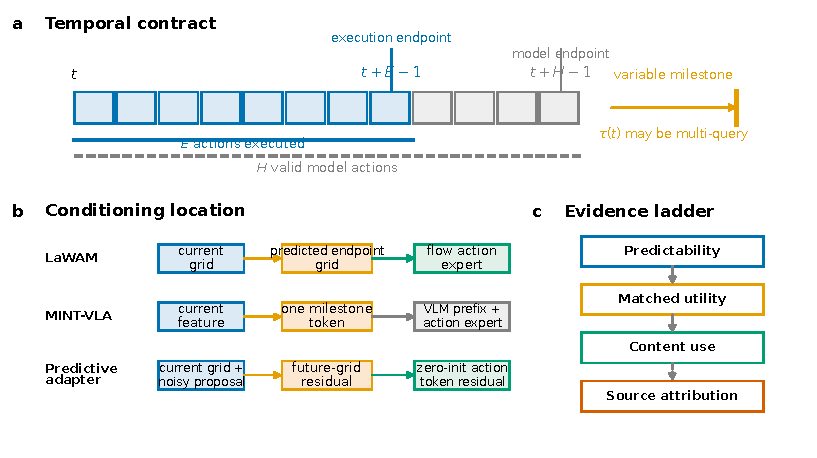
\includegraphics{figures/fig1_contract.pdf}
  \caption{\textbf{Temporal contracts, conditioning interfaces, and evidence
  levels.} \textbf{a}, A VLA predicts $H$ valid actions and executes $E\leq H$
  before replanning.  A target at $\tau(t)$ may coincide with either endpoint
  or lie several queries ahead. \textbf{b}, The evaluated interfaces place a
  predicted future grid in LaWAM's action-expert context, a pooled milestone
  token in the $\pi_{0.5}$ prefix, or a proposal-conditioned residual directly
  on $\pi_{0.5}$ action tokens. \textbf{c}, Prediction, matched utility,
  content use, and source attribution require separate evidence; an arrow
  denotes a required progression, not a logical implication.}
  \label{fig:overview}
\end{figure}

The resulting evidence is asymmetric.  A CPU source audit finds that the
released LaWAM RoboTwin condition is aligned with its 36-action execution
endpoint.  At that frozen checkpoint, normal prediction reaches 94.00\%
success, versus 40.33\% when future content is replaced by a deterministic
within-task, different-episode shuffle.  The +53.67-point paired difference has
a hierarchical 95\% interval of [$+36.08$,$+68.58$], and every task and
evaluation seed is positive.  Null and persistence controls also pass.  Thus
the released policy uses the specific predicted endpoint content in closed
loop.  This fixed-checkpoint intervention does not determine whether the
dependence was created by LaWAM pretraining, downstream auxiliary shaping, or
inference-time conditioning.

The negative cases show why each evidentiary step is necessary.  MINT-VLA
predicts held-out milestones better than persistence but is 8.58 points below
matched no-hint training across three seeds.  PredictiveActionAdapter adds only
0.50\% parameters and passes an offline action-conditioning test, but its
apparent +11.61-point effect against one fixed A0 becomes +1.94 points with a
95\% interval of [$-5.78$,$+12.75$] after independently training all three A0
seeds.  It also contains task regressions and no resolved normal--shuffled
effect.  Finally, changing the executed prefix from 36 to 50 actions does not
produce a local-world-model-specific cadence effect.  Temporal alignment is
therefore a measured distinction and a plausible design hypothesis, not an
established explanation of these outcomes.

This paper makes three contributions:
\begin{itemize}
  \item We formalize the temporal contract between a predicted target, a VLA
  action horizon, and its executed prefix, and define an evidence ladder that
  prevents representation quality or public-system scores from standing in
  for control causality.
  \item We introduce two controlled milestone interfaces, including a
  policy-preserving PredictiveActionAdapter that maps each noisy flow proposal
  to a future-grid residual and an action-indexed correction while retaining
  exact base behavior at initialization.
  \item We provide paired content interventions, independently matched training
  seeds, and task-level safety analyses that establish strong future-content
  use in one released LaWAM checkpoint while rejecting broader utility claims
  for the evaluated MINT-VLA and predictive-adapter instances.
\end{itemize}
          % 1.5 pages
\section{Related Work}\label{sec:related}

\paragraph{Fixed-horizon predicted futures.}
Robot policies condition on future images, video features, or latent
observations at a fixed offset.  VPP uses predictive video representations for
inverse dynamics, WorldVLA generates images and actions autoregressively, and
DreamVLA predicts dynamic, spatial, and semantic scene information
\citep{vpp2024,worldvla2025,dreamvla2025}.  AHEAD predicts future patches in a
frozen OpenVLA space, FutureVLA aligns a joint visuomotor representation with
downstream policies, and $\Delta$VLA represents scene changes relative to the
current observation \citep{ahead2026,futurevla2026,deltavla2026}.  LaWAM uses
an action-conditioned latent model to predict future observation features and
supplies the resulting visual grid to an action expert \citep{lawam2026}.  Our
study does not claim the first future feature, residual prediction, or latent
visual subgoal.  It asks whether the policy uses the specific predicted content
and whether the target time has an explicit relation to the action chunk.

\paragraph{Milestones and long-horizon subgoals.}
Image subgoals can express task progress beyond one controller step.  SuSIE
generates subgoal images for a goal-conditioned controller and compares them
with ground-truth future images \citep{susie2024}; WLA-0 jointly models
subtasks, images, and actions, while Enfold distills a generative model into a
representation inferred from the current observation
\citep{wla02026,enfold2026}.  Recurring states have also been used as
bottlenecks and options \citep{simsek2009,options1999}.  Such targets need not
fall inside the next action chunk.  A distant milestone may support
hierarchical control, but its visual content alone does not specify how much
progress the current chunk should make.

\paragraph{Conditioning interfaces and representation preservation.}
Predicted futures reach the controller through prefix tokens, cross-attention,
latent alignment, or gated feature modulation.  These choices change both the
forward control path and the gradients applied to pretrained features
\citep{dreamvla2025,futurevla2026,deltavla2026}.  Knowledge insulation limits
action-expert gradients into a pretrained VLM \citep{knowledgeinsulation2025},
while auxiliary-task work shows that an extra loss may help or harm a shared
representation independently of its prediction accuracy
\citep{gradsim2018,pcgrad2020,forkmerge2023,lyle2021aux}.  MINT-VLA addresses
target-coordinate drift but retains prefix conditioning.  The
PredictiveActionAdapter instead keeps inherited visual features stop-gradient
and introduces an exactly zero-output route into the action expert.

\paragraph{Evidence for control utility.}
Prediction metrics and decision quality can diverge
\citep{worldarena2026,robowmbench2026,wmevalposition2026}, and correlated
conditioning can create causal confusion in imitation learning
\citep{causalconfusion2019,copycat2020}.  Evaluation seeds quantify rollout
variation for one trained policy; they do not replace independent training
seeds \citep{henderson2018,rliable2021}.  We therefore combine matched training
comparisons with fixed-checkpoint shuffled, null, persistence, and route
interventions.  This design separates a training-package effect from use of the
particular future representation.
        % 1.0 page
\section{Temporal Contracts and Evidence Requirements}\label{sec:setup}

At observation $o_t$ with instruction $l$, a VLA generates $H$ valid actions
\begin{equation}
  A_t=(a_t,\ldots,a_{t+H-1}),
\end{equation}
and executes $E\leq H$ actions before the next query.  Let $\tau(t)$ denote the
frame represented by a future condition $z_t^*=F(o_{\tau(t)})$, and let
$\hat z_t$ be its prediction.  We summarize the target horizon relative to the
model and execution endpoints as
\begin{equation}
 g_t^H=\frac{\tau(t)-t}{H-1},\qquad
 g_t^E=\frac{\tau(t)-t}{E-1}.
\end{equation}
A model-endpoint target has $g_t^H=1$; an execution-endpoint target has
$g_t^E=1$; and a multi-query milestone has $g_t^E>1$.  These definitions
describe timing, not usefulness.  A multi-query target can be effective when a
planner, time-to-go input, or learned hierarchy translates it into a local
action constraint.

The released RoboTwin LaWAM contract has $H=E=36$ and samples its second visual
frame at offset 35.  Its target therefore coincides with both endpoints under
the audited current two-frame loader.  The historical local LMWM contract has
$H=50$ and $E=36$, so its fixed target at offset 49 lies beyond the executed
prefix.  Recurrence milestones vary more strongly: across 420,238 frozen pairs,
their mean horizon is 117.45 frames, only 19.35\% fall within the 50-action
model window, and 12.50\% fall within the executed 36-action prefix.  The
released training stream is unavailable, so endpoint alignment is inferred
from the released config and audited loader rather than reconstructed examples.

We require four levels of evidence:
\begin{enumerate}
  \item \textbf{Predictability:} $\hat z_t$ improves a held-out representation
  metric over persistence or shuffled actions.
  \item \textbf{Matched utility:} independently trained predictive and control
  policies differ in closed-loop success across training seeds.
  \item \textbf{Content use:} at a fixed checkpoint, correct $\hat z_t$
  outperforms paired shuffled content; null and persistence diagnose route and
  future-state dependence separately.
  \item \textbf{Source attribution:} matched component arms isolate
  pretraining, auxiliary shaping, inference conditioning, and their interaction.
\end{enumerate}
No level implies the next.  In particular, representation quality cannot
establish utility, a system score cannot identify a component, and simulator
seeds cannot substitute for training-seed replication.
         % temporal contract and evidence ladder
\section{Predictive Interfaces}\label{sec:method}

\subsection{LaWAM fixed-endpoint conditioning}
LaWAM combines a vision--language model, a frozen latent-action model (LAM),
and a flow-matching action expert \citep{lawam2026}.  The VLM maps current
images and language to a latent-action code.  A LAM decoder combines that code
with the current DINO visual grid to predict a future observation grid.  During
policy training, latent-code distillation and future-grid reconstruction act as
auxiliary objectives.  The flow expert cross-attends to the current grid, the
predicted future grid, and VLM tokens while denoising an action chunk.  At
deployment the future grid is inferred from the current observation; the
future image is not available.

For the released RoboTwin checkpoint, the two-frame training contract samples
the current frame and the last valid frame of its 36-action window.  We call
this the \emph{fixed-endpoint} interface.  Our normal, shuffled, null, and
persistence interventions replace only the predicted future grid after the
checkpoint is loaded.  They therefore test dependence of a fixed policy on the
inference condition, not how that dependence arose during training.

\subsection{Recurrence milestones and MINT-VLA}
MINT-VLA replaces a fixed endpoint with a stage target mined from successful
demonstrations.  It scores cross-episode visual recurrence, divides each
trajectory at score valleys, and maps each frame to the representative of its
next segment or to the terminal frame.  It stores the target image rather than
a stale feature.  During policy training, the current visual encoder
$E_\theta$ represents both images:
\begin{equation}
 c_t=\operatorname{pool}(E_\theta(o_t)),\qquad
 y_t=\operatorname{sg}[\operatorname{pool}(E_\theta(o_{\tau(t)}))].
\end{equation}
A two-layer residual predictor produces
$\hat y_t=c_t+D_\phi(c_t)$ and minimizes
$\|\hat y_t-y_t\|_2^2$.  The evaluated $\pi_{0.5}$ implementation projects
$\hat y_t$ to one bidirectionally visible VLM prefix token.  Recomputing
$y_t$ prevents target-coordinate drift as $E_\theta$ changes, but the target
horizon is variable and the predictor is not action-conditioned.  Stop-gradient
protects only the target branch; the auxiliary loss may still update the
current visual path through $c_t$.

\subsection{Policy-preserving PredictiveActionAdapter}
PredictiveActionAdapter tests a different integration hypothesis: preserve the
pretrained prefix and place an action-conditioned correction inside the action
expert.  Let $C_t\in\mathbb{R}^{16\times d}$ be a stop-gradient $4\times4$
pool of current visual tokens and let
$X=(x_1,\ldots,x_H)$ be an action chunk or flow proposal.  The adapter embeds
each action with a learned temporal position and summarizes the complete
proposal,
\begin{equation}
 u_i=\operatorname{swish}(W_a x_i+p_i),\qquad
 s=\operatorname{swish}(W_s\operatorname{vec}(u_{1:H})).
\end{equation}
It predicts a residual for every visual cell,
\begin{equation}
 \delta_j=W_{p2}\operatorname{swish}
   (W_{p1}[\operatorname{swish}(W_c C_{t,j});s]),\qquad
 \hat C_{t+}=C_t+\delta,
\end{equation}
then summarizes the predicted change and produces one correction per action
token,
\begin{equation}
 \bar\delta=\frac{1}{16}\sum_j\operatorname{swish}(W_c\delta_j),\qquad
 r_i=W_{r2}\operatorname{swish}(W_{r1}[u_i;\bar\delta]).
\end{equation}
The kernel and bias of $W_{r2}$ are initialized to exactly zero, so inserting
the adapter leaves the base policy unchanged at initialization.

Training calls the same adapter twice for different purposes.  A clean expert
action chunk predicts $\hat C_{t+}$ for a cosine loss against a stop-gradient
target grid.  The noisy flow proposal $x_t$ produces $r_{1:H}$, which is added
to the corresponding noisy-action tokens before the action expert predicts the
flow velocity.  At inference no clean action is needed: each denoising step
uses its current proposal $x_t$, recomputes the future-grid residual, and
updates the same proposal through the routed correction.  Temporal reversal,
action masking, and a zero route provide deterministic content and route
interventions.  This makes the adapter a proposal-conditioned self-consistency
interface, not a separate planner or an independently rolled-out world model.

The adapter adds 16.82 million parameters to $\pi_{0.5}$ (0.50\%).  Its
architecture, exact zero-output initialization, and inherited-parameter
isolation are audited.  These properties establish a controlled interface;
control benefit remains subject to the matched-seed, task-safety, and
content-use gates in Section~\ref{sec:results}.
      % predictive interfaces
\section{Experimental Design}\label{sec:design}

\subsection{Benchmark, evaluator, and evidence tiers}
RoboTwin 2.0 is the primary benchmark.  We evaluate hammering, ranking by
color, ranking by size, handover, stacking two blocks, and stacking three
blocks.  Each completed pilot cell contains four simulator seed groups and 50
accepted expert-feasible episodes per group (200 episodes per task and 1,200
per method).  Policies predict 50 actions and replan after executing 36.
Accepted scene identifiers must be intersected across conditions for paired
tests.  LIBERO is reported only as an auxiliary saturation and negative-transfer
diagnostic.

We separate three evidence tiers.  The \emph{external calibration} is the
published $\pi_{0.5}$ checkpoint evaluated through our bridge.  The
\emph{legacy pilot} starts every arm from \texttt{pi05\_base} but uses
joint-delta actions, quantile normalization, batch 64, and 20k updates.  The
\emph{confirmatory matrix} will use absolute actions, mean/std normalization,
batch 16, 50k updates, and the published optimizer schedule for every arm.
Only the confirmatory matrix can support the final Q1 claim.

\subsection{Q1: matched control performance}
The claim-bearing comparison is A0 (no hint), A2-Abs (offline absolute
milestone), and A3/MINT-VLA (current-encoder residual predictor), trained from
the same initialization and data under the confirmatory recipe.  A0 has no
hint field, milestone loss, or milestone-specific parameters.  We will report
each training seed, the seed mean and interval, and all task-level results.

\exptodo{T0--T2}{Finish corrected A0; after its 70\% operational gate, train
matched A2-Abs and six-task-coverage A3 for three independent seeds.}

\subsection{Q2: effect of the predicted token content}
For each trained A2-Abs and A3 checkpoint, we hold weights fixed and replace the
correct prediction with (i) the current-state feature, (ii) zeros, (iii) a
within-task shuffled future, and (iv) a cross-task future.  A completed
feature-dimension permutation is reported separately because it tests feature
structure, not instance relevance.  Conditions use the
same accepted scene identifiers.  Correct-versus-current tests temporal content;
correct-versus-shuffled tests instance relevance while preserving a plausible
feature distribution; zero tests removal of the token; cross-task tests semantic
misdirection.  We report paired success differences and exact McNemar tests
with Holm correction across planned contrasts.
\exptodo{E1}{Complete A3 zero, instance-shuffled, and cross-task conditions;
run the missing A2 instance shuffle; freeze scene intersections and report
discordant counts with Holm-adjusted exact McNemar tests.}

\subsection{Q3: factorized interface mechanism}
The A2-to-A3 pilot changes how target features are computed, predictor capacity, auxiliary
loss, and the injected value at once.  The confirmatory ablation
therefore holds predictor architecture, loss, injected value, and parameter
count fixed while varying one factor:
\begin{center}
\small
\begin{tabular}{p{0.31\linewidth}p{0.55\linewidth}}
\toprule
Factor & Controlled comparison \\
\midrule
target computation & saved target feature vs. frame re-encoded by the current encoder \\
predictor form & direct absolute predictor vs. residual-parameterized predictor, both injecting absolute \\
forward guidance & auxiliary-only/no-prefix vs. predicted prefix \\
backward shaping & prefix-only/no-aux and detached-current auxiliary branch \\
milestone selection & fixed horizon, random future, terminal frame, and oracle milestone \\
\bottomrule
\end{tabular}
\end{center}
\exptodo{T3}{Train the one-factor target-computation, predictor-form, forward/backward
route, capacity, and instruction-aware controls.}

\subsection{Q4: robustness, scope, and efficiency}
Training seed is the top-level uncertainty unit.  We will use a hierarchical
bootstrap over training seed, task, and paired scene, while retaining task-level
values to expose heterogeneous effects.  Transfer is tested by matched
fine-tuning from a mature initialization, not by comparing against an unrelated
public checkpoint.  The task-scope hypothesis is predeclared on block and bowl
stacking, with reactive/contact and fine-grained geometric tasks as controls.
We will also report added parameters, training FLOPs, peak memory, inference
latency, and throughput relative to A0.

Training-seed, mature-initialization, and predeclared task-group experiments
remain confirmatory gates.  We report static deployment cost now and reserve
measured memory and latency claims for a paired benchmark.
\exptodo{T4--T5,E2}{Train the predeclared task panel and mature-initialization
matrix; measure paired peak memory, inference latency, and server throughput.}

\subsection{Q5: instantiation on a second VLA architecture}
The milestone target and predictor are defined independently of the
$\pi_{0.5}$ prefix.  To test use with another architecture, we will retain the
milestone selection, native-space objective, data, and evaluation protocol;
size the predictor to the second VLA's visual feature width; and connect it
through that VLA's native conditioning input.  The identifying comparison is
MINT-VLA versus a matched no-milestone baseline within the second architecture,
not raw success differences between two VLA families.
\exptodo{T6}{Report matched no-milestone and MINT-VLA results for at least one
additional VLA; do not claim multi-architecture evidence from the $\pi_{0.5}$
experiment alone.}
         % experimental design
\section{Results}\label{sec:results}

\subsection{Calibration: the evaluator supports a mature $\pi_{0.5}$}
The published $\pi_{0.5}$ checkpoint obtains \piRTPublic\% on the same six-task,
four-seed bridge (941/1,200 successes): 93.0 hammer, 96.5 ranking-RGB, 64.0
ranking-size, 53.5 handover, 93.5 Stack-2, and 70.0 Stack-3.  This result is an
evaluator calibration, not a matched baseline, because its training mixture and
recipe differ.  The calibration nevertheless shows that the pilot A0 score is mainly
a policy-training issue rather than a globally broken evaluation bridge.

\subsection{Legacy matched pilot: useful signal, insufficient baseline}
Table~\ref{tab:pi05rt} reports the completed legacy pilot.  Every conditioned
method improves its six-task macro over A0.  A2-Abs gains 13.25 points and A3
gains \piRTAThreeVsZero{} points.  However, the absolute success levels remain
far below the public calibration, each row has one training seed, and A3 exceeds
A2-Abs by only \piRTAThreeVsAbs{} points.  We therefore use this result to choose
the confirmatory arms, not as the final MINT-VLA performance claim.

\begin{table}[H]
\centering\small
\caption{Legacy matched $\pi_{0.5}$ RoboTwin pilot: joint-delta actions,
quantile normalization, batch 64, 20k updates.  Each cell averages 200 accepted
episodes; each row has one training seed.}
\resizebox{\linewidth}{!}{%
\begin{tabular}{lrrrrrrr}
\toprule
Method & Hammer & Rank RGB & Rank size & Handover & Stack-3 & Stack-2 & Macro \\
\midrule
A0: no hint & 70.0 & 50.5 & 24.0 & 9.0 & 17.5 & 42.0 & \piRTAZero \\
A1: external absolute & 79.5 & 52.5 & 24.5 & 5.5 & 22.0 & 63.0 & \piRTAOne \\
A2: offline absolute & 78.0 & 65.0 & 30.5 & 19.5 & 30.5 & 69.0 & \piRTATwoAbs \\
A2: offline residual & 76.5 & 52.5 & 34.5 & 18.0 & 25.0 & 56.5 & \piRTATwoResid \\
A3: MINT-VLA current-encoder & 66.0 & 70.5 & 25.5 & 26.0 & 35.5 & 74.0 & \piRTAThree \\
\bottomrule
\end{tabular}}
\label{tab:pi05rt}
\end{table}

The task profile is heterogeneous (Fig.~\ref{fig:pi05tasks}).  A3 improves
ranking-RGB, handover, and stacking but loses on hammer and ranking-size versus
A2-Abs.  Offline residualization is 4.92 points below offline absolute, so
``more change-focused'' is not equivalent to ``more useful as a policy token.''
The A2-to-A3 contrast further changes target computation, predictor capacity, auxiliary
loss, and the injected value; it motivates Q3 but does not identify which factor
caused the difference.

\begin{figure}[H]
  \centering
  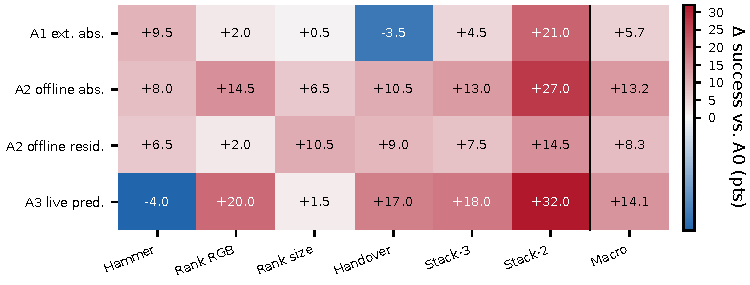
\includegraphics[width=0.88\linewidth]{figures/fig2_redundancy.pdf}
  \caption{Legacy-pilot task deltas relative to A0.  Each cell contains 200
  accepted episodes from one trained checkpoint.  The methods shift
  gains across tasks; none dominates every task.}
  \label{fig:pi05tasks}
\end{figure}

\subsection{The corrected matched comparison is pending}
The corrected A0/A2-Abs/A3 matrix is the primary missing result.  Table
\ref{tab:confirmatory} is intentionally reserved so that pilot numbers cannot
silently become the final baseline.

\begin{table}[H]
\centering\small
\caption{Confirmatory public-recipe RoboTwin matrix.  Report mean and interval
over independent training seeds, plus the full task breakdown.}
\begin{tabular}{lrrr}
\toprule
Method & Train seeds & Six-task macro & $\Delta$ vs. A0 \\
\midrule
A0 no hint & \exptodoid{T0,T2} & \exptodoid{T0,T2} & -- \\
A2 offline absolute & \exptodoid{T1--T2} & \exptodoid{T1--T2} & \exptodoid{T1--T2} \\
A3 MINT-VLA current-encoder & \exptodoid{T1--T2} & \exptodoid{T1--T2} & \exptodoid{T1--T2} \\
\bottomrule
\end{tabular}
\label{tab:confirmatory}
\end{table}

\subsection{The visual token helps, but its predicted future content does not yet}
The five completed A2 conditions do not show that predicted future content
improves control on the
three selected tasks.  Correct, current-state, zero, feature-permuted, and
cross-task content obtain 70.67, 71.00, 67.17, 71.50, and 71.67\% over 600
episodes.  A nonzero visual token helps relative to removing the token, but the
correct prediction is not better than any structured nonzero replacement in
aggregate.  The task profile differs: correct/current/zero are
78.0/73.0/69.5\% on hammer, 65.0/68.5/62.0\% on ranking-RGB, and
69.0/71.5/70.0\% on Stack-2.  Across 179 matched hammer scenes, correct beats
zero in 38 discordant cases and loses in 22 (exact two-sided McNemar
$p{=}0.0519$, before multiplicity correction).  This evidence supports visual
token input but not a general benefit from predicted milestone content.

\begin{table}[H]
\centering\small
\caption{Fixed-checkpoint content intervention.  Final cells use identical
accepted scenes and Holm-adjusted paired tests.}
\begin{tabular}{lrrrrr}
\toprule
Checkpoint & Correct & Current & Zero & Permuted & Cross-task \\
\midrule
A2-Abs & 70.67$^\dagger$ & 71.00$^\dagger$ & 67.17$^\dagger$ & 71.50$^\dagger$ & 71.67$^\dagger$ \\
A3 & 70.17$^\dagger$ & 70.50$^\dagger$ & \exptodoid{E1} & \exptodoid{E1} & \exptodoid{E1} \\
\bottomrule
\end{tabular}
\label{tab:pi05content}
\end{table}
\noindent\footnotesize{$^\dagger$Three-task aggregate over 600 episodes; not
directly comparable to the six-task pilot macro.}\normalsize
\exptodo{E1}{Add within-task instance shuffling for A2; finish A3 zero,
permuted, and cross-task conditions; replace aggregate comparisons with
matched-scene discordant counts and Holm-adjusted tests.}

\subsection{The pilot does not isolate the effect of target recomputation}
No completed comparison holds capacity, target, loss, and injected value fixed
while changing only how the target feature is computed.  Likewise, the current pilot does not
separate forward conditioning from auxiliary representation shaping.
The current evidence therefore supports A3 as an unfactorized
combined integration design, but does not isolate current-encoder target recomputation or residual
parameterization as its cause.

The remaining training matrix tests saved versus recomputed target features,
direct-absolute versus residual-parameterized prediction, auxiliary-only,
prefix-only, detached-current, fixed-horizon, random-future, terminal-frame,
and oracle-milestone controls.
\exptodo{T3}{Populate the factorized mechanism matrix with newly trained,
parameter-matched controls and replicate every claim-bearing contrast.}

\subsection{Task scope and optimization robustness remain unresolved}
The legacy simulator seeds quantify rollout variation around one trained
checkpoint, not optimization variance.  The ordered-construction hypothesis is
also post hoc: on Stack-2/3, legacy A3 averages \piRTStackAThree\% versus
\piRTStackAZero\% for A0, but the public unconditioned checkpoint already
reaches \piRTStackPublic\%.  This may reflect useful stage structure, baseline
room for improvement, or both.  We will make a task-specific claim only if the direction
replicates on predeclared block and bowl stacking, beats a fixed-horizon target
encoded by the current policy, and differs from reactive/contact and geometric control
tasks.

Independent training seeds, matched mature-initialization transfer, and the
predeclared task panel remain pending.  Exact parameter counts and static
predictor FLOPs are reported in the appendix; paired memory and latency
measurements will accompany the confirmatory checkpoints.
\exptodo{T4--T5,E2}{Populate the predeclared scope, mature-transfer, and paired
deployment-cost results.}

\subsection{Use with a second VLA architecture remains to be tested}
The current RoboTwin experiment instantiates MINT-VLA only on $\pi_{0.5}$.  It
tests the one-token prefix implementation, not its use with another VLA
architecture.  A matched experiment on a second VLA is required before the
paper claims evidence beyond the $\pi_{0.5}$ implementation.
\exptodo{T6}{Add a matched second-VLA baseline and MINT-VLA result using the same
milestone construction and evaluation protocol.}

\subsection{Supporting boundary diagnostics}
LaWAM interventions show why Q2 is necessary: correct hints are not reliably
better than zero, instance-shuffled, or cross-task hints, and the former ``no-WM'' arm
inherits WM-aware pretraining and current DINO conditioning.  It is therefore
named \emph{LaWAM-init/Future-off} and used only to diagnose downstream
integration.  LIBERO is similarly auxiliary: its near-saturated four-suite
aggregate is neutral to negative under milestone conditioning.  Full tables
and multiplicity-aware analyses belong in Appendix~\ref{sec:appendix}; neither
diagnostic substitutes for the missing $\pi_{0.5}$ gates.
    % audited evidence and open TG4 gate
\section{Discussion and Conclusion}\label{sec:conclusion}
MINT-VLA improves held-out future-feature prediction, but the corrected
three-seed control experiment rejects action utility: A2-Abs and MINT-VLA are
$-3.94$ and $-8.58$ points below matched no-hint training, respectively.
Correct content also fails to beat fixed-checkpoint replacements.  Oracle stage
transitions, explicit next-subtask semantics, and privileged spatial targets do
not reverse the result.  A later visual state can identify progress without
specifying path, contact, arm assignment, or timing, so predictability and
representation alignment are not sufficient evidence of action sufficiency.

Preserving pretrained pathways does not yield a stable exception.  The
predictive adapter has a strong seed-1000 screen and a positive comparison with
one fixed A0, but independent matched A0s change the three seed effects to
+13.42, -5.50, and -2.08 points (mean +1.94; 95\% CI
[$-5.78$,$+12.75$]).  Its correct-versus-shuffled, route, mature-public, and
task-safety gates also fail.  Recurrence-aligned auxiliary training and
outcome-calibrated weighting provide further negative replication results.

The conclusion is deliberately scoped to the tested $\pi_{0.5}$ milestone and
predictive-adapter interfaces and the six-task RoboTwin panel.  It does not
rule out generative, action-conditioned, spatial, or planning-oriented world
models.  It does show that latent prediction metrics, one-seed gains, and
extra conditioning routes must not substitute for matched training seeds and
causal content controls.
     % 0.5 pages

\subsubsection*{Reproducibility Statement}
The anonymized supplement contains the temporal-contract auditor, frozen
milestone pairs, effective configurations, checkpoint hashes, intervention
mappings, accepted-scene manifests, per-episode outcomes, and canonical JSON
analyses.  TG1A and TG1B include all four conditions and exact pairing checks.
The MINT-VLA and PredictiveActionAdapter packages include all matched training
seeds, task-level effects, intervention reports, and rejected-gate records.
Appendix~\ref{sec:appendix} records protocol boundaries and artifact identities.
No partial rollout or rejected training matrix contributes to a reported
effect.  TG4 artifacts will enter the manuscript only after its joint integrity
and complete-evaluation gates pass.
\exptodo{Archive}{Insert the final anonymous archive URL before submission.}

\subsubsection*{AI Usage Disclosure}
Generative AI tools assisted literature discovery, hypothesis refinement,
experimental design, implementation and code review, figure and table
formatting, drafting and translation, and interpretation of experimental
results.  They were not used to generate demonstrations, simulator outcomes,
or reported measurements.  The authors inspected the relevant source code,
checked configuration and artifact provenance, ran builds and tests, and
verified paper claims against the underlying reports.  The authors take
responsibility for all content and artifacts in this submission.

\bibliography{refs}
\bibliographystyle{iclr2027_conference}

\appendix
\section{Appendix}\label{sec:appendix}

\subsection{Effective configurations}
The completed A0--A3 pilot shares \texttt{pi05\_base}, joint-delta actions,
quantile normalization, 20k updates, batch size 64, and a 50-action horizon.
A0 sets \texttt{lmwm\_hint\_dim=0}.  A1 and A2 use one prefix token with
dimensions 768 and 1152.  A3 uses dimension 1152,
\texttt{lmwm\_live\_hint=True}, \texttt{lmwm\_live\_residual=True}, and
milestone-loss weight 0.05.  The confirmatory configuration instead uses
absolute actions, mean/std normalization, batch 16, 50k updates, and the
published optimizer schedule.  The audited configuration source has SHA-256
\texttt{fe9377c2b93f2428...4dd7264}; the corrected A0 config is
\texttt{pi05\_robotwin\_a0\_public\_recipe\_bj}.  It disables joint deltas and
quantile normalization, uses the \texttt{robotwin2.0\_absolute\_meanstd}
statistics, AdamW weight decay 0.01, batch 16, and 50k updates.  Every
confirmatory arm records its resolved config and dataset-manifest hash next to
its checkpoint rather than relying on the mutable source file.  All nine
A0/A2-Abs/A3 checkpoints at training seeds 1000--1002 finalize step 49,999 and
pass immutable launch, source, checkpoint, dataset, and evaluator audits.  The
accepted scene-manifest SHA-256 is
\texttt{08ed8eb7fa7e166e...9418b820d17}; all protocol checks pass with no
failures.

\subsection{Evaluation and statistics}
Pilot simulator seed groups begin at 100k, 200k, 300k, and 400k.  Candidate
initializations are retained only when the expert planner and benchmark success
check both pass.  Each accepted cohort has 50 episodes per task and seed group.
Because filtering can produce different accepted scenes, intervention tests
use the intersection of scene identifiers.  The completed six-task diagnosis
contains 1,200 paired scenes per method--control comparison and records
discordant counts, exact McNemar tests, and Holm-adjusted $p$-values in
\texttt{logs/l2\_six\_task\_intervention\_analysis.json}.  Confirmatory
training reports include seed-level task cells and hierarchical bootstrap
intervals.  Independently filtered cohorts are never treated as matched
observations.

Each of the nine accepted evaluations uses the frozen confirmatory manifest
and contains all 24 task--evaluation-seed cells.  Seed-level macros are A0:
75.50/80.00/82.67\%, A2-Abs: 70.00/74.67/81.67\%, and A3:
66.92/68.92/76.58\%.  Across training seeds, A0 task means are 89.50 Hammer,
95.00 ranking-RGB, 61.83 ranking-size, 59.83 Handover, 92.83 Stack-2, and 77.33
Stack-3.  A2-Abs changes these by $-3.17$, $-5.83$, $-6.00$, $-5.50$, $+0.50$,
and $-3.67$ points; A3 changes them by $-8.67$, $-6.50$, $-13.00$, $-8.83$,
$-2.83$, and $-11.67$ points.  The paired hierarchical macro differences are
$-3.94$ points for A2-Abs (95\% CI [$-6.58$,$-0.97$]) and $-8.58$ points for A3
([$-11.47$,$-5.75$]), each over 3,600 paired episodes with zero unmatched
episode keys.

The oracle-transition follow-up uses the same three A0 reports and adds three
audited MT1 reports, each with 24 cells and 1,200 episodes.  Oracle macros are
77.75/81.00/81.00\%; paired differences from A0 are
$+2.25$/$+1.00$/$-1.67$ points.  Across training seeds, task differences are
$-1.50$ Hammer, $-0.83$ ranking-RGB, $-1.50$ ranking-size, $+1.67$ Handover,
$+2.17$ Stack-2, and $+3.17$ Stack-3.  The paired hierarchical macro
difference is $+0.53$ points (95\% CI [$-2.06$,$+3.00$]) over 3,600 paired
episodes with zero unmatched keys.  The interval crosses zero, so the
predeclared MT1 gate rejects the oracle-transition branch.

\subsection{Outcome-linked recurrence diagnostics}
The frozen recurrence-diagnostic panel contains 120 public-$\pi_{0.5}$
rollouts: 99 successes and 21 failures across the six RoboTwin tasks.  All 12
task--simulator-seed summaries and 120 videos pass the artifact audit.
Successful-minus-failed terminal progress is 0.11129 (episode-bootstrap 95\%
CI [0.04397,0.18444]) and progress gain is 0.16166
([0.08935,0.24513]).  Failed-minus-successful stall fraction is 0.34827
([0.30419,0.39356]) and regression fraction is 0.12523
([0.02950,0.22978]).  These separations authorize a causal readout test, not a
reward or value claim.  Low density, stall, and regression have success
false-positive rates of 98.99\%, 89.90\%, and 38.38\%, respectively; ranking
RGB has no failed rollout in this panel.  The canonical record is
\texttt{logs/crave\_r0/rollout\_analysis/report.json}.

\subsection{Privileged semantic-subtask protocol}
The semantic screen keeps the public $\pi_{0.5}$ checkpoint, tokenizer,
24-cell scene manifest, replan horizon, and action budget fixed across five
conditions.  Four evaluation seeds contribute 10 episodes per task, for 240
paired episodes per condition.  The primary gate requires the paired 95\%
lower bound for semantic-next minus no-subtask to exceed zero; semantic next
must also exceed generic-stage, semantic-current, and within-task shuffled
semantics in point estimate, with no task regression below $-5$ points.  The
observed semantic-next minus no-subtask difference is $-3.75$ points (95\% CI
[$-10.42$,$+2.92$]), and semantic-next minus shuffled is $-0.42$ points
([$-7.08$,$+6.25$]).  Handover regresses by 25.0 points.  The gate is rejected;
the protocol and final analysis are recorded in
\texttt{manifests/pi05\_r3\_semantic\_screen\_protocol\_v1.json} and
\texttt{logs/r3\_semantic\_screen/report.json}.

\subsection{Recurrence mining}
The mining script (SHA-256 \texttt{d05eefc2f9690163...62c}) applies the following
deterministic procedure independently per task: (1) uniformly retain at most
200 successful episodes; (2) L2-normalize pooled DINOv3 features; (3) set the
RBF bandwidth to the median cross-episode nearest-neighbor distance; (4)
compute the average nearest-match recurrence score; (5) smooth with a temporal
Gaussian of width 1.4; (6) detect valleys with prominence 0.03 and minimum
distance $\max(2,\lfloor T/12\rfloor)$; (7) choose the maximum-recurrence frame
inside each resulting segment; and (8) pair every frame with the next segment's
representative, using the terminal frame in the final segment.  Valley distance
acts as temporal NMS, and selecting one ridge per segment performs within-episode
deduplication.  Cross-episode similarity enters the score rather than a separate
global prototype-clustering stage.

An artifact audit exposed incomplete pilot coverage.  The current
\texttt{pairs.npz} (SHA-256 \texttt{5d68e21fbf0dd462...8ade8}) contains 335,624
pairs from five tasks and omits Stack-3 entirely:
\begin{center}\small
\begin{tabular}{lrrrr}
\toprule
Task & Episodes & Pairs & Unique targets & Future pairs \\
\midrule
Hammer & 200 & 22,820 & 260 & 99.12\% \\
Stack-2 & 200 & 82,204 & 652 & 99.76\% \\
Ranking RGB & 200 & 91,836 & 829 & 99.78\% \\
Ranking size & 200 & 91,932 & 800 & 99.78\% \\
Handover & 200 & 46,832 & 339 & 99.57\% \\
Stack-3 & 0 & 0 & 0 & -- \\
\bottomrule
\end{tabular}
\end{center}
When a pair is absent, the data transform supplies the current image as a
shape-compatible placeholder and sets the milestone-loss mask to false.  The
A3 predictor token remains active through the action loss, but receives no
milestone auxiliary supervision for that sample.  Consequently the legacy
Stack-3 A3 cell measures an added current-state predictor/capacity path, not a
recurrence-supervised milestone.  We therefore generated the frozen
\texttt{robotwin\_milestone\_all6\_confirmatory\_v1} artifact.  It contains 200
episodes for each of the six tasks (1,200 total), including 94,141 Stack-3
pairs; its \texttt{pairs.npz} SHA-256 begins
\texttt{592f1e739105951e}, and its READY audit SHA-256 begins
\texttt{4353c725f7e55f9c}.  It passes nonzero coverage, monotone-target,
selection-manifest, and source-hash checks and is the only recurrence artifact
allowed for confirmatory A3 training.  Threshold sensitivity and alternative
selectors would require newly trained policies, but the positive-utility
prerequisite failed and these expansions are closed.

\subsection{LaWAM mechanism probe}
All diagnostic variants inherit \texttt{lawam\_pretrain}, which contains future
prediction and distillation, and retain current DINO conditioning.  The former
``no-WM'' row is therefore \emph{LaWAM-init/Future-off}, not a clean VLA
baseline.  Across replicated training seeds, Future-off averages 90.83\%
(three seeds), whereas Local future, Absolute, Residual,
Absolute+stop-gradient, and Residual+stop-gradient obtain 86.67, 89.21, 87.50,
89.04, and 88.78\%, respectively.  The latter values use two seeds except
Residual+stop-gradient, which uses three.  Future-off inherits LaWAM-aware
pretraining and therefore does not identify a clean VLA pretraining effect.

At fixed checkpoints, all nine pooled correct-versus-zero, within-task, and
cross-task comparisons have Holm-adjusted $p{=}1$.  The adverse Handover
contrast for Residual+stop-gradient is 72.5\% correct versus 82.5\% with a
same-task foreign-instance hint (Holm-adjusted $p{=}0.0337$).  These data
diagnose downstream future conditioning but do not replace the corrected
$\pi_{0.5}$ A0/A2/A3 comparison.

\subsection{Exploratory task groups and LIBERO boundary}
In the legacy Stack-2/3 subset, A0, A2-Abs, A2-Res, and A3 average 29.75, 49.75,
40.75, and 54.75\%.  The public no-hint checkpoint reaches 81.75\%.  This
post-hoc two-task pattern is not a validated applicability law.  The
predeclared extension covers block and bowl stacking and includes reactive and
geometric controls.

The auxiliary $\pi_{0.5}$ LIBERO diagnostic uses checkpoint step 29,999,
OSMesa rendering, three rollout seeds, and the same one-prefix-token interface:
\begin{center}\small
\begin{tabular}{lrrr}
\toprule
Suite & A0 & A1 DINO & A2 So400m \\
\midrule
LIBERO-10 & 94.7 & 94.3 & 92.7 \\
Goal & 96.7 & 97.3 & 97.3 \\
Object & 98.7 & 100.0 & 100.0 \\
Spatial & 99.7 & 99.3 & 98.7 \\
\midrule
Four-suite macro & 97.42 & 97.75 & 97.18 \\
\bottomrule
\end{tabular}
\end{center}
The aggregate deltas are +0.33 and -0.24 points.  Thirty of forty A0 tasks
already exceed 97\%, so this table is a saturation/boundary diagnostic rather
than primary support for MINT-VLA.  The task-type split observed inside LIBERO-10
(ordered closures positive, unordered collection negative) is exploratory and
is tested prospectively in Q4 rather than promoted from these small cells.

\subsection{Efficiency and reproducibility}
Parameter trees constructed from the resolved Flax NNX models give the exact
counts below.  A3's two $2048\!\times\!2048$ linear layers add 8.39M MACs
(approximately 16.78 MFLOPs under the two-FLOP convention) per predictor call,
excluding the small attention cost of one additional prefix token.
\begin{center}\small
\begin{tabular}{lrrr}
\toprule
Arm & Parameters & Added vs. A0 & Relative \\
\midrule
A0 & 3,353,433,872 & -- & -- \\
A1 & 3,355,008,784 & 1,574,912 & 0.047\% \\
A2 & 3,355,795,216 & 2,361,344 & 0.070\% \\
A3 & 3,361,826,576 & 8,392,704 & 0.250\% \\
\bottomrule
\end{tabular}
\end{center}
Under the matched four-A100 training protocol, A0, A2-Abs, and A3 peak at
67,247, 67,247, and 67,265 MiB, respectively; A3 adds 18 MiB (0.027\%).  Their
paired core inference latencies are 57.19, 58.35, and 57.99 ms, and end-to-end
WebSocket latencies are 107.20, 108.91, and 107.01 ms.  Corresponding
throughputs are 9.33, 9.18, and 9.34 requests/s.  These measurements show no
material A3 deployment penalty relative to A0; they do not establish a speed
advantage over other world-model-augmented policies.

The implementation environment pins Python 3.11, JAX 0.5.3 with CUDA 12,
Flax 0.10.2, and PyTorch 2.7.1.  The audited workspace revision is
\texttt{8d28087d2f69d063...2d01270e}; because the experiment tree contains
uncommitted research changes, file hashes above are the authoritative
identifiers.  Pilot rollout seed groups start at 100k, 200k, 300k, and 400k.
The confirmatory launch manifests, reports, and paired scene audit are recorded
with the accepted checkpoints and summarized in
\texttt{RESULTS\_pi05\_confirmatory\_3seed\_2026-08-02.md}.  The AI-use
disclosure appears in the main paper.


\end{document}
